%%%%%%%%%%%%%%%%%%%%%%%%%%%%%%%%%%%%%%%%%%%%%%%%%%%%%%%%%%%%%%%%%%%%%
% LaTeX Template: Project Titlepage Modified (v 0.1) by rcx
%
% Original Source: http://www.howtotex.com
% Date: February 2014
% 
% This is a title page template which be used for articles & reports.
% 
% This is the modified version of the original Latex template from
% aforementioned website.
% 
%%%%%%%%%%%%%%%%%%%%%%%%%%%%%%%%%%%%%%%%%%%%%%%%%%%%%%%%%%%%%%%%%%%%%%

\documentclass[12pt]{article}
\usepackage[a4paper]{geometry}
\usepackage[myheadings]{fullpage}
\usepackage{fancyhdr}

\usepackage{lastpage}
\usepackage{graphicx, wrapfig, subcaption, setspace, booktabs}
\usepackage[utf8]{inputenc}
\usepackage[T1]{fontenc}
%\usepackage[font=small, labelfont=bf]{caption}
\usepackage{fourier}
\usepackage[protrusion=true, expansion=true]{microtype}
\usepackage[french]{babel}
\usepackage{sectsty}
\usepackage{url, lipsum}


\newcommand{\HRule}[1]{\rule{\linewidth}{#1}}
\onehalfspacing
\setcounter{tocdepth}{5}
\setcounter{secnumdepth}{5}

%-------------------------------------------------------------------------------
% HEADER & FOOTER
%-------------------------------------------------------------------------------
\pagestyle{fancy}
\fancyhf{}
\setlength\headheight{15pt}
\fancyhead[L]{Emmanuel Debezenac, Arthur Ramolet}
\fancyhead[R]{UPMC}
\fancyfoot[R]{\thepage\ / \pageref{LastPage}}
%-------------------------------------------------------------------------------
% TITLE PAGE
%-------------------------------------------------------------------------------

\begin{document}

\title{ \normalsize \textsc{COMPLEX}
		\\ [2.0cm]
		\HRule{0.5pt} \\
		\LARGE \textbf{\uppercase{Ordonnancement de tâches sur des machines en série}}
		\HRule{2pt} \\ [0.5cm]
		\normalsize \today \vspace*{5\baselineskip}}

\date{}

\author{
		Emmanuel Debezenac, Arthur Ramolet \\ 
		Université Pierre et Marie Curie \\
		Année Universitaire 2015-2016 }

\maketitle

\newpage
\tableofcontents

\newpage
%-------------------------------------------------------------------------------
% Section title formatting
\sectionfont{\scshape}
%-------------------------------------------------------------------------------


%----------------------------------------------------------------------------------------
%	INTRO
%----------------------------------------------------------------------------------------
\clearpage
\newpage
\section{Introduction}



%----------------------------------------------------------------------------------------
%	PART 1
%----------------------------------------------------------------------------------------
\clearpage
\newpage
\section{Algorithme approché avec garantie de performance}


%------------------------------------------------

\subsection{3-Approché}

Pour montrer que l'ordonnancement associé à P, une permutation arbitraire est 3-approché, il faudrait montrer que : \\
\begin{center}
(1) $Cout(P) \le \displaystyle\sum_{i=1}^n(d_i^A+d_i^B+d_i^C)$\\
\end{center}
\begin{center}
(2) $OPT \ge \frac{1}{3}\displaystyle\sum_{i=1}^n(d_i^A+d_i^B+d_i^C)$\\
\end{center}
(1) et (2) nous donne bien :\\
\begin{center}
$3OPT \ge \displaystyle\sum_{i=1}^n(d_i^A+d_i^B+d_i^C) \ge Cout(P)$\\
\end{center}
=> l'ordonnancement associé à P serait 3-approché\\

Montrons (1) : $Cout(P) \le \displaystyle\sum_{i=1}^n(d_i^A+d_i^B+d_i^C)$\\

$\displaystyle\sum_{i=1}^n(d_i^A+d_i^B+d_i^C)$ correspond à la date de fin des taches \{1,...,n\} lorsqu'on est obligé d'attendre que la tache i soit terminée sur la machine C avant de commencer la tache i+1 sur la machine A. Cela reviendrait à exécuter toutes les taches sur une seule machine (Au niveau de la date de fin, et en supposant qu'une machine puisse exécuter les taches des machines (A,B,C)). \\

En pratique, lorsque la tache i sur la machine A (respectivement B) est terminée on peut commencer directement la tache i+1 sur la machine B (respectivement C).\\

Remarque : Nous avons l'égalité lorsqu'il n'y a qu'une seule tache à effectuer.\\

Montrons maintenant (2) :\\

$\frac{1}{3}\displaystyle\sum_{i=1}^n(d_i^A+d_i^B+d_i^C)$ est la durée moyenne de travail des machines A,B,C sur les taches \{1,...,n\}. Il y a forcément une machine qui prend d'avantage de temps à effectuer ses taches que la durée moyenne :\\
\begin{center}
(3) $\frac{1}{3}\displaystyle\sum_{i=1}^n(d_i^A+d_i^B+d_i^C) \le \max(\displaystyle\sum_{i=1}^n d_i^A,\displaystyle\sum_{i=1}^n d_i^B,\displaystyle\sum_{i=1}^n d_i^C)$\\
\end{center}
Comme toute les taches doivent passer sur chaque machine, nous avons :\\
\begin{center}
(4) $\max(\displaystyle\sum_{i=1}^n d_i^A,\displaystyle\sum_{i=1}^n d_i^B,\displaystyle\sum_{i=1}^n d_i^C) \le OPT$\\
\end{center}
avec (3) et (4) nous avons :\\
\begin{center}
$\frac{1}{3}\displaystyle\sum_{i=1}^n(d_i^A+d_i^B+d_i^C) \le OPT$\\

=> P est 3-approché.
\end{center}
Exemple : Soit $\epsilon$ > 0, 3 taches de durées :\\
\begin{center}
\begin{tabular}{|c|c|c|c|}
\hline 
Tache/Machine & A & B & C \\ 
\hline 
1 & $\epsilon$ & $\epsilon$ & 1 \\ 
\hline 
2 & $\epsilon$ & 1 & $\epsilon$ \\ 
\hline 
3 & 1 & $\epsilon$ & $\epsilon$ \\ 
\hline 
\end{tabular} 
\end{center}
Cas OPT :

(Image)

Lorsque $\epsilon$ -> 0, durée de fin = 1. avec permutation (1,2,3).

Cas WSPT :

(Image)

Lorsque $\epsilon$ -> 0, durée de fin = 3. avec permutation (3,2,1).

\subsection{2-Approché}

Soit $D_i^j$ la date de fin d'ordonnancement t retournée par l'algorithme de Johnson appliqué sur i machines.
Nous pouvons montrer l'inégalité suivante : \\
\begin{center}
$D_3^J \le D_2^j + \displaystyle\sum_{i=1}^n d_i^C$\\
\end{center}
Nous avons bien que la date de fin d'ordonnancement de 3 machines est au moins aussi bonne que la date sur 2 machines, plus les taches à effectuer sur la machine C.\\

De plus, (*) $D_2^j \le OPT_3$ ($OPT_3$ étant la date de fin d'ordonnancement sur 3 machines, car $D_2^j \ge OPT$ est optimale sur 2 machines, et ou ne prends pas en compte les taches $D_i^C$).\\

Nous avons aussi (**)$\displaystyle\sum_{i=1}^n d_i^C \le OPT_3$ (car il y a au minimum la première tache de la machine A $D_i^A$ qui devrait être prise en compte).\\
\begin{center}
Donc :
$D_3^J \le D_2^j + \displaystyle\sum_{i=1}^n d_i^C \le 2OPT$ avec (*) et (**)
\end{center}
Exemple : Soit $\epsilon$ > 0, 3 taches de durées :\\
\begin{center}
\begin{tabular}{|c|c|c|c|}

\hline 
Tache/Machine & A & B & C \\ 
\hline 
1 & $\epsilon$ & 1 & $\epsilon$ \\ 
\hline 
2 & $\epsilon$ & $\epsilon$ & 1 \\ 
\hline 
3 & 1 & $\epsilon$ & $\epsilon$ \\ 
\hline 
\end{tabular} 
\end{center}
L'algorithme de Johnson nous renverrait la permutation (1,2,3), ce qui nous donne :

(Image)

OPT : Permutation (2,1,3)

(Image)

=> 2-approché, au mieux.

\subsection{Implémentation}

Pour traiter cette partie nous avons choisi le langage C. La gestion "A la main" de la mémoire en permet une utilisation optimale, de plus le langage étant proche de la machine et notre compilateur (GCC) permettant l'optimisation du code via des flags (On utilisera -02 pour notre projet) nous garantie des performances accrues par rapport à un langage plus haut niveau. \\

Le développement sous GNU/Linux nous permet également d'utiliser facilement le timestamp UNIX afin de chronométrer nos temps d'exécution avec une précision raisonnable (En théorie, en microsecondes. En pratique, pour de petites instances le temps est difficile a évaluer à cause des nombreuses opérations des différents algorithmes, donc plutôt de l'ordre de la dixième de microseconde (À la louche)).\\

Nous avons implémenté deux versions différentes de l'algorithme de Johnson afin de comparer leurs performances. La première version est celle fournie dans le sujet. La seconde est la même avec tri des taches afin d'en optimiser le comportement. La première version possède une complexité en O($n^2$) la seconde O(n Log n).On teste nos algorithmes pour des instances dont le nombre de tache évolue de 1 à 2500, celles-ci sont générées aléatoirement selon 3 classes : Données non-corrélées, Corrélation sur les durées d'exécution et Corrélation sur les machines.\\

\begin{figure}[!ht]
\centering
\centerline{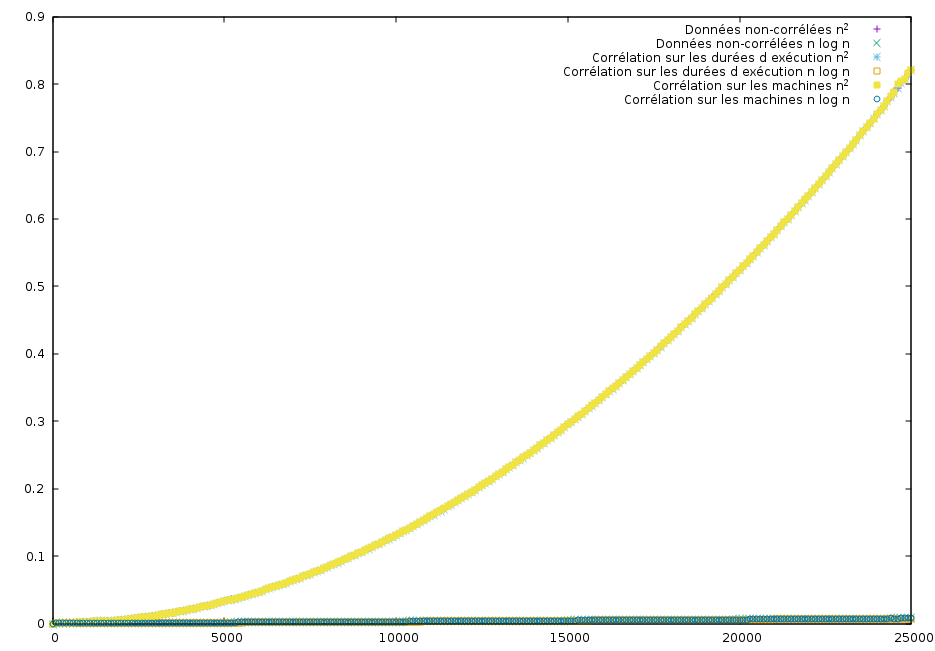
\includegraphics[scale=0.7]{johnson.png}}
\caption{Temps de calcul des algorithmes de johnson et des différentes classes de génération d'instance.}
\label{john}
\end{figure}

On observe que l'algorithme de Johnson avec tri propose de bien meilleurs performances que l'algorithme original.
Celui-ci étant 2-approché, il pourra être utilisé afin de trouver une borne supérieure de notre instance.
On observe aussi que les différentes classes n'influent pas sur le déroulement de l'algorithme. (Les courbes sont confondues pour chaque classe).

%----------------------------------------------------------------------------------------
%	Part 2
%----------------------------------------------------------------------------------------
\clearpage
\newpage
\section{Méthode exacte}

\subsection{Première borne}

Montrons que dans $b_B^\pi$, on peut remplacer $t_B^\pi$ par :
(formule 12), c'est à dire $t_B^\pi \ge {t^\prime}_B^\pi$ (On cherche la plus grande borne inférieure).

(Cas 1)

Ici, une fois les taches $\pi$ terminées sur A, on rajoute la tache i, $i\in{\pi}^\prime,i = {\arg\min\limits_{i\in{\pi^\prime}}}\{d_A^i\}$, pour ne pas perdre de généralité.

Ici, $t_A + d_A^i < t_B$. Il faudra alors attendre que les taches de $\pi$ se terminent sur B avant de pouvoir commencer i sur B.

(Cas 2)

Ici, $t_A + d_i^A \ge t_B$. Il faudra donc attendre i sur A avant de commencer i sur B.

Au lieu d'uniquement prendre en compte $t_b^\pi$ pour la borne inférieur, ce serait plus efficace de prendre en compte au moins une durée en plus (ici $\min\limits_{i\in{\pi^\prime}}\{d_A^i\}$, car elle pourrait nous donner une borne inférieure plus grande (Cf cas 2).

=> On remplace donc $t_B^\pi$ par $\max\{t_B^\pi,\min\limits_{i\in{\pi^\prime}}\{d_A^i\}+t_A^\pi\}$.


Montrons maintenant, qu'on peut toujours obtenir une borne inférieure en remplaçant $t_C^\pi$ par ${t^\prime}_C^\pi$ :

-> On va faire un raisonnement analogue à (la première borne) qui consiste à chercher les taches contraignantes. On va également choisir les taches de durée minimale, pour ne pas perdre de généralité ($\forall$ permutation de $\pi^\prime$, on aura toujours au moins le minimum).

(cas 1)

(cas 2)

(cas 3)

En optant pour les durées les plus grandes on construit une borne inférieure plus précise. En choisissant la tache minimale comme la première tache on ne perds pas de généralité car on cherche une borne inférieure. (si la tache $i\in\pi^\prime$ est contraignante sur la machine $j\in\{A,B,C\}$, toutes les taches de $\pi^\prime$ le seraient également).

=> On peut remplacer $t_C^\pi$ par ${t^\prime}_C^\pi$, tel que :\\
\begin{center}
${t^\prime}_C^\pi = \max\{t_C^\pi,t_B^\pi + \displaystyle\min_{i \in \pi^\prime} d_B^i, t_A^\pi + \displaystyle\min_{i \in \pi^\prime}\{d_A^i + d_B^i\}\}$
\end{center}

\subsection{Deuxième borne}

On schématise cette situation; pour simplifier, on suppose les taches \{1,...,k-1,k,k+1,...,n\} tel que : $d_i^A \le d_i^C, \forall i \in \{1,...,k-1\}$ et $d_i^A > d_i^C, \forall i \in \{k+1,...,n\}$

(Figure)

Pour simplifier, on suppose que les taches $\pi$ des machines B et C ne sont pas contraignantes (si elles l'était, on aurait un temps total plus grand). Pour que l'ordonnancement soit tel que sa date de fin soit égal à :\\
\begin{center}
$t_A^\pi + \displaystyle\sum_{d_A^i \le d_C^i}d_A^i + d_A^k + d_B^k + d_C^k + \displaystyle\sum_{d_A^i > d_C^i}d_C^i$\\
\end{center}
, il faudrait faire les suppositions fortes que les taches \{1,...,k\} soient contraignantes sur la machine A (Alors que par définition, on a $d_A^i \le d_C^i$), c'est à dire que ces mêmes taches ne soient pas contraignantes pour les machines B et C, aussi que la supposition que les taches \{k+1,...,n\} soient contraignantes sur la machine C (alors que $d_i^A > d_i^C, \forall i \in \{k+1,...,n\}$.

On a que $\forall k \in \pi^\prime$ la date de fin d'ordonnancement associé à P est supérieure ou égale à cette borne inférieure. Donc pour trouver une borne inférieure, nous avons la liberté de choisir notre k, la meilleur option serait donc de choisir un k qui maximise notre borne, c'est à dire :\\
\begin{center}
 $b2 = t_A^\pi + \displaystyle\max_{k \in \pi^\prime}\{d_A^k + d_B^k + d_C^k + \displaystyle\sum_{i \in \pi^\prime,d_A^i \le d_C^i} d_A^i + \displaystyle\sum_{i \in \pi^\prime,d_A^i > d_C^i} d_C^i\} $\\
\end{center}
\subsection{Troisième borne}

En faisant le même raisonnement, on peut déduire la borne :\\


\begin{center}


 $b3 = t_B^\pi + \displaystyle\max_{k \in \pi^\prime}\{d_B^k + d_C^k + \displaystyle\sum_{i \in \pi^\prime,d_B^i \le d_C^i} d_B^i + \displaystyle\sum_{i \in \pi^\prime,d_B^i > d_C^i} d_C^i\} $\\
\end{center}

(Figure)

\subsection{Implémentation}

Pour traiter cette partie nous avons choisi le même langage pour les mêmes raisons que précédemment. Ainsi que pour une réutilisation aisée de l'algorithme de Johnson.\\

Ayant opté pour une implémentation récursive du branch and bound, celle-ci diffère un peu de celle vue en cours. Le cœur récursif de l'implémentation se charge d'effectuer toute les permutations possibles, à chacune de ses permutations, on calcule une borne supérieure et une borne inférieure. Celles-ci déterminent si oui ou non, l'exploration doit se poursuivre dans la branche courante, comme traité en TD pour un problème de minimisation. Nous avons choisi l'implémentation récursive car elle nous paraissait plus intuitive pour un parcours d'arbre et utilisant l'optimisation de GCC, la récursion est traité comme une boucle avec une pile. En soit, après optimisation, le code doit fonctionner de la même façon que l'algorithme étudié en cours. 

L'algorithme pouvant difficilement traiter des instances à plus de 10 taches, ce sera notre taille maximale durant les tests. Les moyennes ont été calculées sur 200 tests.

\begin{figure}[!ht]
\centering
\centerline{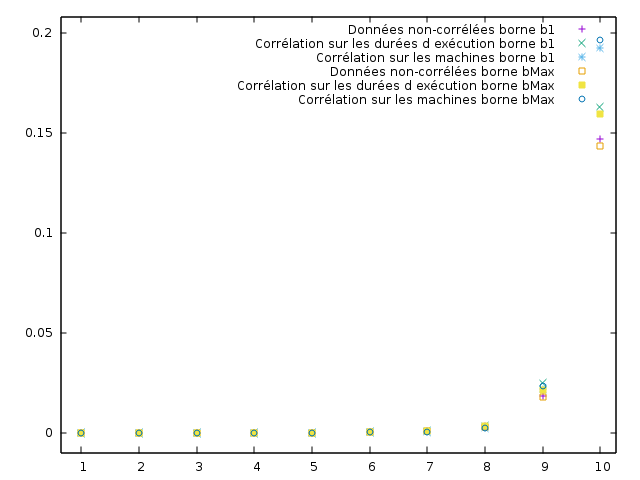
\includegraphics[scale=0.9]{tempsmoyen.png}}
\caption{Temps de calcul moyen pour pour les bornes b1 et bMax ainsi que des différentes classes de génération d'instance.}
\label{tmpmoy}
\end{figure}

\begin{figure}[!ht]
\centering
\centerline{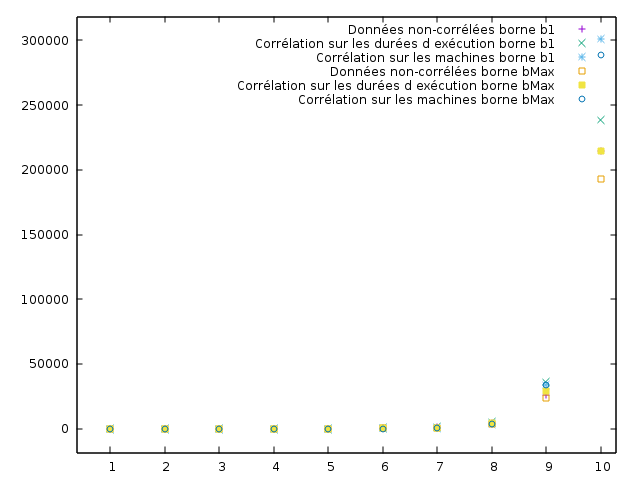
\includegraphics[scale=0.9]{nodemoyen.png}}
\caption{Nombre moyen de noeuds explorés pour les bornes b1 et bMax ainsi que des différentes classes de génération d'instance.}
\label{ndmoy}
\end{figure}




%------------------------------------------------



%----------------------------------------------------------------------------------------

%----------------------------------------------------------------------------------------
%	PART 3
%----------------------------------------------------------------------------------------
\clearpage
\newpage
\section{Méthode de recherche arborescente approchée}

\subsection{Possibilités}


\subsection{Implémentation}


%------------------------------------------------
\clearpage
\newpage
\section{Conclusion}


%Figure : \ref{pouthisteqr}

%\newpage
%\begin{figure}[!t]
%\centering
%\centerline{\includegraphics{moon.jpg}}
%\caption{L'image moon.tif.}
%\label{moontif}
%\end{figure}



\end{document}
